\documentclass[11pt]{article}
\usepackage[T1]{fontenc}
\usepackage[margin=1in]{geometry}
\usepackage{amsmath,amssymb}
\usepackage{graphicx}
\usepackage{booktabs}
\usepackage{longtable}
\usepackage{array}
\usepackage{xcolor}
\usepackage{tikz}
\usetikzlibrary{arrows.meta,positioning,fit,backgrounds}
\usepackage[colorlinks=true,linkcolor=blue!60!black,urlcolor=blue!60!black,
            citecolor=blue!60!black]{hyperref}
\usepackage[htt]{hyphenat}
\usepackage{microtype}
\emergencystretch=3em
\usepackage{listings}
\lstset{basicstyle=\ttfamily\footnotesize, backgroundcolor=\color{gray!8},
        frame=single, rulecolor=\color{gray!40}, breaklines=true,
        columns=fullflexible, keepspaces=true, showstringspaces=false,
        numbers=left, numberstyle=\tiny\color{gray}, language=C++}

\newcommand{\code}[1]{\texttt{#1}}
\newcommand{\file}[1]{\texttt{\small #1}}
\newcommand{\fn}[1]{\texttt{\small #1}}
\newcommand{\St}{S}
\newcommand{\ts}{t_{\rm s}}
\newcommand{\rhod}{\rho_{\rm d}}
\newcommand{\rhog}{\rho_{\rm g}}
\newcommand{\vf}{v_{\rm frag}}

\newcommand{\invariant}[2]{%
  \par\vspace{0.6em}\noindent
  \fcolorbox{gray!40}{gray!8}{\parbox{0.97\linewidth}{\textbf{#1}\quad #2}}%
  \par\vspace{0.6em}}

\title{Dust Growth on Superparticles in AthenaK\\[0.4em]
       \large \textsc{Implementation Document}\\
       \large D1: the growth step; D2: diagnostics; the \code{nsh\_init} option of
       \code{streaming\_strat}}
\author{worktree \code{athenak-worktrees/dust-growth}, branch \code{dust-growth}
        (parent \code{9aaa5639})\\
        \small commits \code{a821cb4d} (growth step, diagnostics, tests) and
        \code{e231fc7f} (\code{nsh\_init}, R1 set-up)}
\date{October 19, 2026}

\begin{document}
\maketitle

\begin{abstract}
\noindent
This document explains, file by file and line by line, how dust growth and
fragmentation were added to the AthenaK dust module for the NHFP 2027 preliminary
result (the streaming instability with live dust growth in a stratified box). The design
is the simplest one that makes every existing kernel grow-aware without touching it:
each superparticle keeps its mass and carries the size of the grains it represents in
its stopping time \code{IPTS}, which every drag kernel already reads per particle. Once
per cycle, before anything else in the time step, an operator-split growth step
deposits the dust density, gathers it and the gas velocity at each particle, and
advances \code{IPTS} by the Birnstiel et al.\ (2012) two-population law for equal-size
sticking, reversing sign where the collision speed exceeds the fragmentation velocity.
The document derives the law, places the step in the time loop and the task graph,
walks through the kernel, lists every other part of the code that sees the changed
stopping times (drag, timestep, gamma switch, restart, migration, AMR), and documents
the diagnostics, the inputs and the limitations. A companion document
(\file{dust\_growth\_validation.pdf}) reports the tests.
\end{abstract}

\tableofcontents
\newpage

%=========================================================================================
\section{Scope and how to read this}

\subsection{What this document is}
It is the reference for the code added on branch \code{dust-growth}: the growth step
(\file{src/dust/dust\_growth.cpp}, task D1 of \file{HANDOFF\_DUST\_GROWTH.md}), the
diagnostics that make the grown sizes visible (D2), and the NSH initial condition added
to \code{streaming\_strat} for the R1 production runs. Section~\ref{sec:physics}
derives the physics; Sections~\ref{sec:loop}--\ref{sec:kernel} follow one cycle through
the code; Section~\ref{sec:consumers} lists everything else that reads the stopping
time; Sections~\ref{sec:diag}--\ref{sec:inputs} are the diagnostics and parameter
reference; Section~\ref{sec:limits} states what the model does not do.
Appendix~\ref{app:source} reproduces \file{dust\_growth.cpp} in full.

\subsection{Files touched}
\begin{longtable}{>{\raggedright}p{0.36\linewidth}p{0.58\linewidth}}
\toprule
file & change \\
\midrule
\file{src/dust/dust\_growth.cpp} (new) & \fn{InitGrowth}, the \fn{GrowthStep} task,
  the \fn{GrowStoppingTimes} kernel \\
\file{src/dust/dust.hpp} & enum \code{DustGrowth}; growth parameters and counters as
  members of \code{DustGasDrag}; task id \code{id.growth}; the three declarations \\
\file{src/dust/dust.cpp} & \fn{InitGrowth(pin)} called from the constructor;
  \code{DUST\_GROWTH\_SUMMARY} in the destructor \\
\file{src/dust/dust\_tasks.cpp} & \fn{GrowthStep} added to
  \code{before\_timeintegrator}, with \fn{GammaSwitch} depending on it \\
\file{src/CMakeLists.txt} & \file{dust/dust\_growth.cpp} added to the sources \\
\file{src/outputs/particle\_history.cpp}, \file{outputs.hpp} & Stokes-number columns
  of the \code{phst} output when growth is on \\
\file{src/outputs/vtk\_prtcl.cpp} & \code{SCALARS ptaus} in the particle VTK when the
  stopping times are per particle \\
\file{src/pgen/tests/streaming\_strat.cpp} & opt-in \code{<problem>/nsh\_init}
  (Section~\ref{sec:nsh}) \\
\file{inputs/dust/dust\_growth\_box.athinput} & the D3 test box \\
\file{inputs/dust/streaming\_strat\_growth\_r1.athinput} & the R1 production input \\
\file{scripts/analysis/dust\_growth\_tests.\{sh,py\}},
\file{dust\_growth\_tests\_fig.jl}, \file{si\_growth\_r1\_fig.jl} & test suite, checker,
  figures \\
\file{scripts/cluster/build\_growth\_h2.slurm}, \file{si\_growth\_r1\_h2.slurm} & h-2
  build and run scripts \\
\bottomrule
\end{longtable}

\invariant{Invariant.}{With \code{<dust>/growth = none} (the default) the new task
returns immediately and nothing else changes: every output of the parent commit is
reproduced byte for byte (test (a) of the validation document). The only visible
difference is the extra line \code{growth = none} that AthenaK echoes into the parameter
block of restart files.}

%=========================================================================================
\section{Design: why the stopping time carries the size}\label{sec:design}

\subsection{The representative-particle convention}
A superparticle stands for a swarm of identical grains. In the representative-particle
method (Zsom \& Dullemond 2008; the basis of \code{mcdust}, Dr\k{a}\.zkowska et al.\
2014) the swarm mass is fixed and the grains in it grow: the number of grains per swarm
falls as each grain gets heavier. This is what the code does: the particle mass
\code{IPM} never changes, and the grain size changes.

\subsection{Why the stopping time and not a new field}
AthenaK's dust particles have 17 real fields (\file{src/particles/particles.cpp}:99):
positions, velocities, their RK registers, the recorded drag rates, the stopping time
\code{IPTS} (index 15) and the mass \code{IPM} (16), declared in
\file{src/athena.hpp}:79. In Epstein drag at fixed gas density the stopping time is
proportional to the grain size, so \code{IPTS} \emph{is} the size up to a constant. The
dust module already reads \code{IPTS} per particle in every drag kernel (listed in
Section~\ref{sec:consumers}); changing it between steps therefore makes the whole
integrator respond to growth with no change to any drag, deposit or solver code. A new
size field would have needed a conversion in every one of those kernels.

\subsection{The constant-Stokes convention}
Shearing-box SI calculations fix the dimensionless stopping time $\tau_s=\Omega\ts$
rather than the size, i.e.\ they evaluate the Epstein law at a reference gas density
$\rho_{\rm g0}$ (the midplane density) instead of the local one. The growth code keeps this
convention: the Stokes number of a particle is
\begin{equation}
  \St = \Omega\,\ts \qquad\text{(at } \rhog=\rho_{\rm g0}\text{)},
\end{equation}
so a particle high in the atmosphere has the same $\ts$ as one of the same size at the
midplane. Code units are $\rho_{\rm g0}=H=\Omega=c_s=1$ in every input used here, so
$\St=\ts$ numerically; the code nevertheless keeps $\Omega$, $c_s$ and $\rho_{\rm g0}$ as
explicit parameters (Section~\ref{sec:inputs}).

\subsection{The \code{stopping\_time\_mode} contract}
The dust module has three modes (\file{dust.hpp}:46):
\code{species\_fixed} (every particle's \code{IPTS} must equal its species value
\code{taus\_s}), \code{particle\_static} (arbitrary positive per-particle values that
never change) and \code{dynamic} (values may change; their global maximum and minimum
are refreshed every cycle). Growth changes \code{IPTS}, so \fn{InitGrowth} refuses to
run unless the mode is \code{dynamic}. The modes are enforced by
\fn{RefreshStoppingTimeMaximum} (\file{dust\_newdt.cpp}:34), which aborts if any
\code{IPTS} is non-finite or non-positive, or (in \code{species\_fixed}) differs from its
species value; it runs once at start-up in the first two modes and every cycle in
\code{dynamic}.

%=========================================================================================
\section{The physics of the growth law}\label{sec:physics}

\subsection{From sticking to a scale-free law}
For Epstein drag the stopping time of a grain of radius $a$ and material density
$\rho_s$ is
\begin{equation}
  \ts = \frac{\rho_s a}{\rhog v_{\rm th}},\qquad v_{\rm th}=\sqrt{8/\pi}\,c_s ,
\end{equation}
so at the reference density
\begin{equation}
  \St = \sqrt{\frac{\pi}{8}}\,\frac{\rho_s a\,\Omega}{\rho_{\rm g0} c_s}. \label{eq:St}
\end{equation}
Equal-size sticking: a grain of mass $m=\frac43\pi\rho_s a^3$ sweeps grains of the same
size with cross section $\sigma=\pi(2a)^2$ at relative speed $\Delta v$ through a dust
density $\rhod$, gaining mass at $\dot m=\rhod\sigma\Delta v$. With
$\dot m=4\pi\rho_s a^2\dot a$ this is
\begin{equation}
  \frac{da}{dt} = \frac{\rhod\,\Delta v}{\rho_s},
\end{equation}
the growth rate of Birnstiel et al.\ (2012, with sticking efficiency 1). Inserting into
\eqref{eq:St}:
\begin{equation}
  \boxed{\;\frac{d\St}{dt} = \sqrt{\frac{\pi}{8}}\;\Omega\;\frac{\rhod}{\rho_{\rm g0}}\;
  \frac{\Delta v}{c_s}\;}
  \qquad\Longleftrightarrow\qquad
  \frac{d\ts}{dt} = \sqrt{\frac{\pi}{8}}\;\frac{\rhod}{\rho_{\rm g0}}\;\frac{\Delta v}{c_s}.
  \label{eq:law}
\end{equation}
The grain material density cancels: the law needs no $\rho_s$ and no physical units.
The code integrates the second form, so $\Omega$ enters only through the turbulent
speed below. A physical size for figures follows from \eqref{eq:St} with
$\Sigma_g=\sqrt{2\pi}\rho_{\rm g0}H$:
\begin{equation}
  a = \frac{2}{\pi}\,\frac{\St\,\Sigma_g}{\rho_s}.
\end{equation}

\subsection{Collision speeds}
Two sources, added in quadrature:
\begin{equation}
  \Delta v^2 = \Delta v_{\rm turb}^2 + \Delta v_{\rm drift}^2 .
\end{equation}
\begin{description}
\item[Turbulence.] $\Delta v_{\rm turb}=\sqrt{3\alpha_t\St}\,c_s$, the
  intermediate-regime expression of Ormel \& Cuzzi (2007) used by Birnstiel et al.\
  (2012). $\alpha_t$ (\code{growth\_alpha}) is a \emph{prescribed} parameter: the box
  contains no imposed turbulence, so $\alpha_t$ represents unresolved turbulence and is
  not measured from the flow (Section~\ref{sec:limits}).
\item[Differential drift.] $\Delta v_{\rm drift}=\frac12|\mathbf v_p-\mathbf
  u_g(\mathbf x_p)|$, with $\mathbf v_p$ the particle velocity and $\mathbf u_g$ the gas
  velocity interpolated to the particle. For $\St\ll1$ the velocity of a grain relative
  to the gas is proportional to $\St$, so the partner of half the size moves at half the
  relative speed and the two differ by half of $|\mathbf v_p-\mathbf u_g|$. Because
  $\mathbf v_p$ and $\mathbf u_g$ are the \emph{actual} local velocities, this term
  includes radial drift, azimuthal drift and settling as the simulation produces them,
  including their modification by back-reaction and by the SI. It can be switched off
  (\code{growth\_drift = false}).
\end{description}

\subsection{Fragmentation}
Where $\Delta v>\vf$ (\code{growth\_vfrag}, in units of $c_s$) the right-hand side of
\eqref{eq:law} changes sign: grains shrink at the rate they would have grown (the
simple form of Vericel et al.\ 2021). With turbulence alone this caps the Stokes number
at
\begin{equation}
  \St_{\rm frag} = \frac{\vf^2}{3\alpha_t c_s^2}\qquad
  \bigl(\alpha_t=10^{-4},\ \vf=0.01c_s:\ \St_{\rm frag}=0.33;\quad
  \alpha_t=10^{-3}:\ 0.033\bigr).
\end{equation}
Birnstiel et al.\ (2012) multiply this by a safety factor $f_f\approx0.37$; the code
does not. The particles then dither around the cap with an amplitude of one step's
change. Drift alone caps where $\frac12|\Delta\mathbf v|=\vf$; for a dust-poor gas
$|\Delta\mathbf v|\approx2\St\Pi c_s$, giving $\St\approx\vf/(\Pi c_s)=0.2$ for
$\vf=0.01c_s$, $\Pi=0.05$. Back-reaction reduces the relative drift by about
$1/(1+\epsilon)$ in a dust-rich layer, which raises the drift cap there.

\subsection{Connection to the two-population growth time}
In a settled Gaussian layer of thickness $H_d=H\sqrt{\alpha_t/(\alpha_t+\St)}$ the
midplane dust density is $\rhod=Z\rho_{\rm g0}H/H_d$. With turbulent collisions and
$\St\gg\alpha_t$, \eqref{eq:law} gives
\begin{equation}
  \frac{d\St}{dt}=\sqrt{\frac{3\pi}{8}}\,Z\,\Omega\,\St
  \quad\Rightarrow\quad
  t_{\rm grow}=\frac{\St}{d\St/dt}\approx\frac{0.92}{Z\Omega},
\end{equation}
the size e-folding time of the Birnstiel et al.\ (2012) two-population model. The
superparticle law reproduces it where the layer is in that equilibrium, and does
something more general where it is not (each particle sees its own local $\rhod$ and
$\Delta v$).

%=========================================================================================
\section{Where the step sits in a cycle}\label{sec:loop}

\subsection{The driver loop}
\fn{Driver::Execute} (\file{src/driver/driver.cpp}:533) runs, every cycle:
\begin{enumerate}
\item the task list \code{before\_timeintegrator} (stage 0, line 565);
\item for each RK stage: \code{before\_stagen}, the Poisson solve (if
  \code{<gravity>}), \code{stagen}, \code{after\_stagen};
\item \code{after\_timeintegrator};
\item $t\to t+\Delta t$, \code{ncycle++};
\item outputs (\fn{LoadOutputData}/\fn{WriteOutputFile}, line 628);
\item adaptive mesh refinement (line 634);
\item \fn{Mesh::NewTimeStep} (line 636): the $\Delta t$ of the \emph{next} cycle.
\end{enumerate}
The growth step is the first task of item~1, so it acts on the state that was just
written to disk and uses the $\Delta t$ that the coming cycle will take.

\begin{figure}[h]
\centering
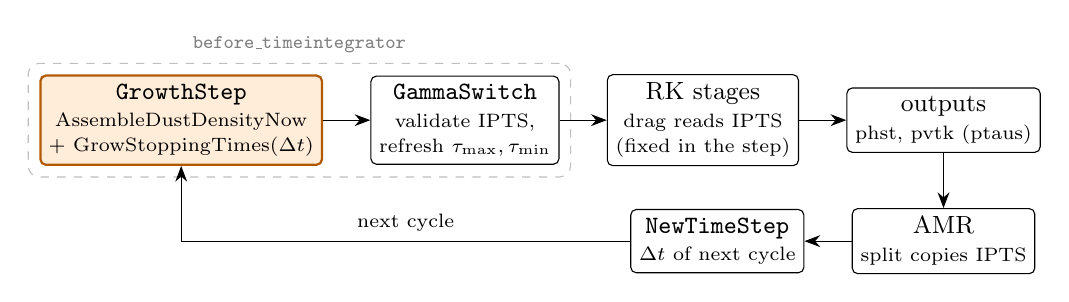
\begin{tikzpicture}[node distance=4mm and 6mm, every node/.style={font=\small},
  box/.style={draw, rounded corners=2pt, align=center, minimum height=8mm,
              inner sep=3pt, fill=white},
  new/.style={box, fill=orange!15, draw=orange!70!black, thick},
  arr/.style={-{Stealth[length=2mm]}}]
\node[new] (grow) {\fn{GrowthStep}\\[-1pt]\scriptsize AssembleDustDensityNow\\[-2pt]
  \scriptsize + GrowStoppingTimes($\Delta t$)};
\node[box, right=of grow] (gsw) {\fn{GammaSwitch}\\[-1pt]\scriptsize validate IPTS,\\[-2pt]
  \scriptsize refresh $\tau_{\max},\tau_{\min}$};
\node[box, right=of gsw] (stages) {RK stages\\[-1pt]\scriptsize drag reads IPTS\\[-2pt]
  \scriptsize (fixed in the step)};
\node[box, right=of stages] (out) {outputs\\[-1pt]\scriptsize phst, pvtk (ptaus)};
\node[box, below=7mm of out] (amr) {AMR\\[-1pt]\scriptsize split copies IPTS};
\node[box, left=of amr] (dt) {\fn{NewTimeStep}\\[-1pt]\scriptsize $\Delta t$ of next cycle};
\draw[arr] (grow) -- (gsw);
\draw[arr] (gsw) -- (stages);
\draw[arr] (stages) -- (out);
\draw[arr] (out) -- (amr);
\draw[arr] (amr) -- (dt);
\draw[arr] (dt.west) -| node[pos=0.25, above, font=\scriptsize]{next cycle} (grow.south);
\begin{scope}[on background layer]
\node[draw=gray!50, dashed, rounded corners, fit=(grow)(gsw), inner sep=4pt,
      label={[font=\scriptsize, gray]above:\code{before\_timeintegrator}}] {};
\end{scope}
\end{tikzpicture}
\caption{One cycle. The new task (orange) runs first; \fn{GammaSwitch} depends on it.}
\label{fig:cycle}
\end{figure}

\subsection{The task}
\file{dust\_tasks.cpp}:44--48:
\begin{lstlisting}[numbers=none]
id.growth  = tl["before_timeintegrator"]->AddTask(&DustGasDrag::GrowthStep,this,none);
id.gswitch = tl["before_timeintegrator"]->AddTask(&DustGasDrag::GammaSwitch,this,
                                                  id.growth);
\end{lstlisting}
Before this change \fn{GammaSwitch} depended on nothing. The dependency guarantees
the order growth $\to$ validation; the task is added unconditionally and returns
immediately when \code{growth = none}.

\subsection{Why first, and why once per cycle}
\begin{itemize}
\item \textbf{The stopping time must not change inside a step.} The imex2+ integrator
  records drag rates at one implicit stage and applies them at the next (the
  \code{a\_twid} history term, \code{IPRX}--\code{IPRZ}); the hybrid PC2 and split-BE
  paths also assume one $\ts$ per step. All of this is consumed within one cycle, so a
  change between cycles is safe and a change between stages would not be.
\item \textbf{The derived quantities must be refreshed after the change.}
  \fn{GammaSwitch} calls \fn{RefreshStoppingTimeMaximum} first thing (in
  \code{dynamic} mode), which validates the new values and recomputes $\tau_{\max}$
  (used by the imex2+ $\gamma$ switch, Krapp et al.\ 2024 eq.~18) and $\tau_{\min}$ (used
  by the hybrid coupling to choose PC2 or split-BE). Running growth before it means
  both are always computed from the stopping times the step will actually use.
\item \textbf{Operator splitting.} The step is a first-order (Lie) split: growth over
  $\Delta t$ from the start-of-cycle state, then the full dynamics over $\Delta t$ with
  fixed $\ts$. The splitting error is $O(\Delta t/t_{\rm grow})$ per unit time; in the
  production runs $\Delta t\approx2\times10^{-4}\Omega^{-1}$ against
  $t_{\rm grow}\gtrsim10\,\Omega^{-1}$. Test (b) of the validation document measures
  the first-order convergence.
\end{itemize}

%=========================================================================================
\section{Set-up: \fn{InitGrowth}}\label{sec:init}
Called from the \code{DustGasDrag} constructor (\file{dust.cpp}:453) after the
stopping-time mode, the EOS and the shearing-box parameters have been read, because it
needs all three. In order (\file{dust\_growth.cpp}:58--117):
\begin{enumerate}
\item \code{<dust>/growth} is \code{none} (return; every growth member keeps its default
  from \file{dust.hpp}) or \code{monodisperse}; anything else is a fatal error.
\item \code{stopping\_time\_mode} must be \code{dynamic} (fatal otherwise).
\item \code{growth\_alpha} and \code{growth\_vfrag} are read with \fn{GetReal}, so they
  are \emph{required}: there is no sensible default for either.
\item \code{growth\_smin} ($10^{-5}$), \code{growth\_smax} (1), \code{growth\_maxfrac}
  (0.05), \code{growth\_drift} (true), \code{growth\_rho0} (1) have defaults;
  \code{growth\_omega} defaults to \code{<shearing\_box>/omega0} in a shearing box and to
  1 otherwise; \code{growth\_cs} defaults to the isothermal sound speed and is required
  for an ideal gas (whose sound speed varies).
\item Validation: $\alpha_t\ge0$, $\vf>0$, $0<\St_{\min}<\St_{\max}$, positive cap,
  $\rho_{\rm g0}$, $\Omega$, $c_s$.
\item Rank 0 prints one line with the law, the parameters and $\St_{\rm frag}$.
\end{enumerate}

%=========================================================================================
\section{The step: \fn{GrowthStep}}\label{sec:step}
\begin{lstlisting}[firstnumber=125]
TaskStatus DustGasDrag::GrowthStep(Driver *pdrive, int stage) {
  if (growth == DustGrowth::none) {return TaskStatus::complete;}
  // collective (ghost exchanges): every rank, every cycle, even without particles
  AssembleDustDensityNow();
  GrowStoppingTimes(pmy_pack->pmesh->dt);
  return TaskStatus::complete;
}
\end{lstlisting}

\subsection{Assembling the dust density}
The kernel needs $\rhod$ at each particle. Particle-mesh interpolation with the TSC
kernel reads a $3\times3\times3$ block of cells around the particle, which reaches one
cell into the ghost zone for a particle near a MeshBlock edge, so the density must be
complete in the active zone \emph{and} correct in the first ghost layer.
\fn{AssembleDustDensityNow} (\file{dust\_gravity.cpp}:288), written for the
self-gravity source and the \code{dust\_dpm} output, does exactly this, synchronously:
\begin{enumerate}
\item \fn{DepositMass} (line 78): zero \code{rho\_dust}; scatter
  $m_pW(\mathbf x-\mathbf x_p)/V$ with the module's deposit kernel (TSC by default) into
  the active cells and the ghost cells. On a refined mesh every block deposits with the
  kernel of the finest level present, through a fine image that is then volume-averaged
  onto the block (\fn{DepositStencil}, \fn{RestrictImage}), so the density is one
  consistent field across level jumps.
\item Additive exchange (\code{pbval\_rd}): each block sends the mass it deposited into
  its ghost cells to the neighbour that owns those cells, which adds it to its active
  cells. After this the active zone holds the complete density.
\item Shear fold (\fn{FoldShearDeposit}): across a shear-periodic $x_1$ face the
  neighbour's cells are offset in $y$ by $q\Omega L_xt$, so the ghost deposits are
  remapped conservatively in $y$ before being added.
\item Copy exchange (\code{pbval\_rc}) and its shear remap (\code{psbox\_rc}): now that
  every active cell is complete, the ghost layer is overwritten with the neighbours'
  active values (prolongated next to coarser neighbours on a refined mesh).
\end{enumerate}
Every step is collective, so \fn{GrowthStep} calls it on every rank, every cycle,
including ranks without particles; the ordering of collectives is the same on all ranks
because \code{before\_timeintegrator} executes its tasks in a fixed order.

At physical (non-periodic) faces nothing fills the ghost layer from outside; there it
keeps the block's own ghost deposits. That only matters for particles within a cell of
such a face (never the case in the periodic-$z$ R1 box).

\subsection{The cost}
One extra deposit and three exchanges per cycle. Measured: $\approx1\%$ in the YJ14 box
on 4 Mac ranks, and $\approx7.5\%$ in the R1 box on 64 h-2 ranks, where the comparison
also includes the per-cycle \code{MPI\_Allreduce}s of \code{dynamic} mode.

%=========================================================================================
\section{The kernel: \fn{GrowStoppingTimes}}\label{sec:kernel}
One Kokkos \code{parallel\_reduce} over the particles of the rank; the three reduction
variables count how often the cap, the clamp and fragmentation act.

\subsection{Constants (lines 156--165)}
\begin{lstlisting}[firstnumber=156]
  const Real coef = std::sqrt(M_PI/8.0)/(growth_rho0*growth_cs);  // d t_s/dt per rho_d dv
  const Real turb = 3.0*growth_alpha*growth_omega*SQR(growth_cs);  // dv_turb^2 per t_s
  const Real vfrag = growth_vfrag*growth_cs;
  const Real tsmin = growth_smin/growth_omega, tsmax = growth_smax/growth_omega;
\end{lstlisting}
\code{coef} is the prefactor of the $\ts$ form of \eqref{eq:law}, so that
$\dot\ts=\code{coef}\cdot\rhod\cdot\Delta v$. \code{turb} is $3\alpha_t\Omega c_s^2$, so
that $\Delta v_{\rm turb}^2=\code{turb}\cdot\ts=3\alpha_t\St c_s^2$. The Stokes limits
are converted to stopping-time limits once. Class members are copied into local
\code{const}s because a device lambda cannot capture \code{this}.

\subsection{Interpolation weights (lines 170--183)}
\fn{PMWeights} (\file{dust.hpp}:149) is the same helper every drag kernel uses: for a
coordinate it returns the index of the nearest cell (\code{ip}) and three weights for
cells \code{ip-1}, \code{ip}, \code{ip+1} (NGP, CIC or TSC by \code{<dust>/deposit}).
Gathers always use the block's own cells (on a refined mesh, unlike deposits, there is
no fine image), exactly as in \fn{GatherKickPMBR}. In 2D only $x_1,x_2$ are weighted.

\subsection{The gather (lines 185--204)}
\begin{lstlisting}[firstnumber=185]
    Real rd = 0.0, ux = 0.0, uy = 0.0, uz = 0.0;
    ...
          rd += w*rhod(m,0,kk,jj,ii);
          ux += w*w0(m,IVX,kk,jj,ii);
          Real vy = w0(m,IVY,kk,jj,ii);
          if (full) {
            vy += qo*(mbsize.d_view(m).x1min + (static_cast<Real>(ii - is) + 0.5)*dx1);
          }
          uy += w*vy;
          uz += w*w0(m,IVZ,kk,jj,ii);
\end{lstlisting}
\begin{description}
\item[The dust density] comes from \code{rho\_dust}, just assembled. It contains every
  particle's mass, including the particle's own swarm (spread by its kernel). That is
  the representative-particle convention (Zsom \& Dullemond 2008): a representative
  grain collides with grains of every swarm in its neighbourhood, its own included.
\item[The gas velocity] comes from the primitive array \code{w0}. At the start of a
  cycle \code{w0} is valid in the active zone and in all ghost cells: the previous
  stage ended with the boundary exchange, the physical boundary conditions and
  \fn{ConToPrim} over the whole array, and the first stage of the coming cycle needs
  those ghosts for its fluxes anyway. The drag kernels gather a different field (the
  provisional velocity $u^\ast$ of the implicit solve), which does not exist yet at
  this point of the cycle; \code{w0} is the end-of-step gas velocity.
\item[Frames.] Particle velocities are always shear-relative. With orbital advection
  (FARGO) the gas velocities are too. Without it (\code{gas\_full\_frame}, 3D only) the
  gas $v_y$ includes the background shear $-q\Omega x$, and the kernel adds back
  $+q\Omega x$ at each stencil cell's centre: the same shift \fn{ShiftGasFrame}
  (\file{dust\_frame.cpp}) applies to the gas momenta for the drag tasks. Because TSC
  weights reproduce linear functions exactly ($\sum w_a=1$, $\sum w_a x_a=x_p$), the
  interpolated shift equals $q\Omega x_p$ to round-off, so the frame correction is
  exact. In the 2D $r$--$z$ shearing box the azimuthal components are \code{IVZ} and
  \code{IPVZ}, and they are paired consistently by component index.
\end{description}

\subsection{The rate and its limits (lines 205--227)}
\begin{lstlisting}[firstnumber=205]
    Real ts = pr(IPTS,p);
    Real dv2 = turb*ts;
    if (drift) {
      dv2 += 0.25*(SQR(pr(IPVX,p) - ux) + SQR(pr(IPVY,p) - uy) + SQR(pr(IPVZ,p) - uz));
    }
    Real dv = sqrt(dv2);
    Real rate = coef*fmax(rd, 0.0)*dv;
    if (dv > vfrag) {
      rate = -rate;
      frag += 1;
    }
    Real dts = rate*dt;
    Real lim = maxfrac*ts;
    if (fabs(dts) > lim) {
      dts = (dts > 0.0) ? lim : -lim;
      cap += 1;
    }
    Real tsn = ts + dts;
    if (tsn < tsmin || tsn > tsmax) {
      tsn = fmin(fmax(tsn, tsmin), tsmax);
      clamp += 1;
    }
    pr(IPTS,p) = tsn;
\end{lstlisting}
\begin{itemize}
\item $\Delta v^2=3\alpha_t\St c_s^2+\frac14|\mathbf v_p-\mathbf u_g|^2$; the drift
  term uses all three components.
\item \code{fmax(rd,0)} guards against a negative interpolated density (not possible
  with TSC weights and positive masses, but cheap).
\item Forward Euler over $\Delta t$: $\ts\to\ts+\dot\ts\Delta t$.
\item \textbf{Cap} (\code{growth\_maxfrac}): no particle changes its $\ts$ by more than
  this fraction in one cycle. In normal operation it never binds (the per-step change
  is $\sim\Delta t/t_{\rm grow}\sim10^{-5}$); it exists so that a pathological input
  (huge $\alpha_t$ or $\rhod$) cannot produce a negative or exploding $\ts$ in one step.
  When it binds, the result depends on $\Delta t$, so the count is reported.
\item \textbf{Clamp} (\code{growth\_smin}, \code{growth\_smax}): a hard floor and
  ceiling on $\St$. A particle sitting at a limit is counted every cycle.
\item The new value overwrites \code{IPTS} in place; nothing else about the particle
  changes.
\end{itemize}

\subsection{Counters}
The three reduction results are added to rank-local \code{unsigned long long} totals
(\code{growth\_capped}, \code{growth\_clamped}, \code{growth\_frag}); the destructor
sums them over ranks and rank 0 prints
\begin{lstlisting}[numbers=none]
# DUST_GROWTH_SUMMARY steps=N capped=.. clamped=.. fragmenting=.. (particle-steps; ...)
\end{lstlisting}
(\code{steps} is the number of growth steps of rank 0).

%=========================================================================================
\section{Everything else that sees the stopping time}\label{sec:consumers}

\subsection{The drag kernels (unchanged)}
\begin{longtable}{>{\raggedright}p{0.30\linewidth}p{0.62\linewidth}}
\toprule
where & use of \code{IPTS} \\
\midrule
\file{dust\_push.cpp}:186, 224--226 & hybrid PC2: implicit-midpoint factor
  $\lambda=\frac12\Delta t/\ts$ and the drag impulse $\Delta t(u-v)/\ts$ \\
\file{dust\_push.cpp}:306--308 & hybrid split-BE: $c_j=\Delta t/(\ts+\Delta t)$ and the
  deposited rate $m/(\ts V)$ \\
\file{dust\_pm.cpp}:114 & imex2+ deposit of $Q=\sum m/(\ts V)$ for the per-cell solve \\
\file{dust\_pm.cpp}:180, 403 & imex2+ gather--kick: $c_j=a\Delta t/(\ts+a\Delta t)$ \\
\file{dust\_solver.cpp}:177, 504, 558 & coupled solvers (PCG, adaptive) \\
\bottomrule
\end{longtable}
All of them read the value per particle and per stage, so they use the grown value from
the cycle after it was set. None constrains the timestep: AthenaK's dust integrators are
stable for any $\Delta t/\ts$, so growth to large $\ts$ or a floor at small $\ts$ never
changes $\Delta t$.

\subsection{Validation and derived maxima}
\fn{RefreshStoppingTimeMaximum} (\file{dust\_newdt.cpp}:34), called by
\fn{GammaSwitch} right after the growth step, aborts the run if any \code{IPTS} is
non-finite or $\le0$ (so a bug in growth cannot silently corrupt a run), then sets
$\tau_{\max}$ and $\tau_{\min}$ with two global reductions.

\subsection{Migration, restart, AMR}
\begin{itemize}
\item \textbf{Migration} between MeshBlocks and ranks packs all \code{nrdata} real
  fields of a particle (\file{bvals/bvals\_part.cpp}:577--589), so \code{IPTS} travels
  with the particle.
\item \textbf{Restart} files write and read all \code{nrdata} fields
  (\file{outputs/restart.cpp}:273, 645); a restarted run continues bitwise (test (e)).
\item \textbf{AMR splitting}: when a block refines with
  \code{<particles>/split\_on\_refine}, each particle becomes $2^d$ children that copy
  all real fields of the parent and get $1/2^d$ of its mass
  (\file{particles/particles\_amr.cpp}:133--150); children carry the parent's grown
  \code{IPTS} (test (e), split check).
\end{itemize}

%=========================================================================================
\section{Diagnostics (D2)}\label{sec:diag}

\subsection{Particle history (\code{phst})}
When growth is on, \fn{ParticleHistoryOutput} appends six columns after the
per-species ones: \code{St\_mean} (mass-weighted mean of $\St=\Omega\ts$),
\code{St\_max}, \code{St\_min}, and the mass fractions \code{fm\_St>0.01},
\code{fm\_St>0.03}, \code{fm\_St>0.1}. One more \code{parallel\_reduce} with four sums,
a max and a min; sums are reduced over ranks with \code{MPI\_SUM}, the extrema with
\code{MPI\_MAX}/\code{MPI\_MIN}. With growth off the file is unchanged.

\subsection{Particle VTK}
\fn{ParticleVTKOutput} writes a \code{SCALARS ptaus} block (after the integer scalars,
before \code{VECTORS pvel}) whenever \code{stopping\_time\_mode} is not
\code{species\_fixed}. In \code{species\_fixed} runs the stopping time follows from
\code{pspecies}, and the historical schema and I/O volume are kept. Readers that locate
blocks by keyword (\file{baehr\_table1.py}, \file{dust\_growth\_tests.py},
\file{si\_growth\_r1\_fig.jl}) are unaffected by the extra block.

%=========================================================================================
\section{The NSH initial condition of \code{streaming\_strat}}\label{sec:nsh}
For R1 the stratified-SI generator gained \code{<problem>/nsh\_init} (default false; with
it false the generator's output is bitwise unchanged). Lim et al.\ (2025, ApJ 981, 160)
start gas and particles at the Nakagawa et al.\ (1986) drift equilibrium for the local
dust-to-gas ratio; without it a dust-rich midplane starts out of force balance and
sloshes radially.

For one species with $\tau=\Omega\ts$ and the radial forcing $a_x=2\Omega\eta v_K$ on the
gas (\code{etavk} $=\eta v_K$), the steady shear-relative velocities solve
\begin{align}
 0&=2\Omega u_y+a_x+\epsilon(v_x-u_x)/\ts, &
 0&=-(2-q)\Omega u_x+\epsilon(v_y-u_y)/\ts,\\
 0&=2\Omega v_y-(v_x-u_x)/\ts, &
 0&=-(2-q)\Omega v_x-(v_y-u_y)/\ts ,
\end{align}
whose solution for general $q$ is, with $D=(1+\epsilon)^2+2(2-q)\tau^2$,
\begin{equation}
 v_x=-\frac{2\tau\eta v_K}{D},\quad v_y=-\frac{(1+\epsilon)\eta v_K}{D},\quad
 u_x=\frac{2\epsilon\tau\eta v_K}{D},\quad
 u_y=-\frac{(1+\epsilon+2(2-q)\tau^2)\eta v_K}{D}
\end{equation}
(the familiar Keplerian form for $q=3/2$). The local ratio is
$\epsilon(z)=\rho_p(z)/\rhog(z)$ with $\rhog=\rho_{\rm g0}e^{-z^2/2H^2}$ and, for the Gaussian
layer of width $h_z$ truncated to the box (the generator's particle placement),
$\rho_p(z)=Z\Sigma_g e^{-z^2/2h_z^2}/(\sqrt{2\pi}h_zf)$, where $f$ is the fraction of
the Gaussian inside the box ($\rho_p=Z\Sigma_g/L_z$ for a uniform layer). Gas cells use
$\epsilon$ at their centre, particles at their own height; vertical velocities are zero;
\code{gas\_vy0} is ignored. Only one species is supported (fatal otherwise). With
orbital advection off, the background shear is added to the gas momentum as before.

%=========================================================================================
\section{Input reference}\label{sec:inputs}
\begin{longtable}{>{\raggedright}p{0.26\linewidth}>{\raggedright}p{0.17\linewidth}p{0.49\linewidth}}
\toprule
parameter (\code{<dust>}) & default & meaning \\
\midrule
\code{growth} & \code{none} & \code{none} or \code{monodisperse} \\
\code{stopping\_time\_mode} & \code{species\_fixed} & must be \code{dynamic} with growth \\
\code{growth\_alpha} & required & $\alpha_t$ of $\Delta v_{\rm turb}=\sqrt{3\alpha_t\St}c_s$ \\
\code{growth\_vfrag} & required & $\vf/c_s$ \\
\code{growth\_smin}, \code{growth\_smax} & $10^{-5}$, 1 & clamp on $\St$ \\
\code{growth\_maxfrac} & 0.05 & largest fractional change of $\ts$ per cycle \\
\code{growth\_drift} & true & include $\frac12|\mathbf v_p-\mathbf u_g|$ \\
\code{growth\_rho0} & 1 & $\rho_{\rm g0}$ of the Stokes number and of \eqref{eq:law} \\
\code{growth\_omega} & \code{omega0} (or 1) & $\Omega$ in $\St=\Omega\ts$ and in
  $\Delta v_{\rm turb}$ \\
\code{growth\_cs} & \code{iso\_sound\_speed} & $c_s$ (required for an ideal gas) \\
\midrule
\code{<problem>/nsh\_init} & false & \code{streaming\_strat}: NSH velocities for the local
  $\epsilon(z)$ \\
\bottomrule
\end{longtable}
Initial stopping times come from \code{<dust>/taus\_s} through the problem generator as
before; growth starts from whatever \code{IPTS} the generator wrote.

%=========================================================================================
\section{Limitations and what comes next}\label{sec:limits}
\begin{itemize}
\item \textbf{Locally monodisperse.} Each particle grows as if every grain within its
  kernel had its own size: the partner density is the total $\rhod$ and the relative
  speed is that of equal (turbulence) or half-size (drift) partners. Particles of
  different sizes in the same cell do not collide with each other's actual sizes. A
  Monte Carlo collision step between superparticles (the \code{mcdust} approach) is the
  Year-1 deliverable that removes this.
\item \textbf{Prescribed $\alpha_t$.} $\Delta v_{\rm turb}$ uses a parameter, while the
  box has only SI-driven turbulence. The dust layer is therefore thinner, and $\rhod$
  higher, than in a real disk with the same $\alpha_t$, which makes growth faster. A
  self-consistent alternative (task D4) is $\Delta v$ from the resolved local particle
  velocity dispersion.
\item \textbf{Constant-Stokes convention.} $\ts$ is evaluated at $\rho_{\rm g0}$, not at the
  local gas density, as in SI calculations without growth.
\item \textbf{Sharp fragmentation switch} without the $f_f$ safety factor or a smooth
  transition; particles at the cap dither by one step's change.
\item \textbf{First-order splitting} (Section~\ref{sec:loop}); the error is negligible
  at production timesteps but visible in the deliberately coarse test (b).
\item \textbf{Cost:} one extra deposit and exchange per cycle (1--8\% measured). A
  \code{growth\_interval} that accumulates $\Delta t$ over several cycles would reduce it
  if needed.
\end{itemize}

%=========================================================================================
\appendix
\section{\file{src/dust/dust\_growth.cpp}}\label{app:source}
\lstinputlisting{../src/dust/dust_growth.cpp}

\end{document}
